% -*- mode: latex -*-

\week{Data}

Get out a piece of paper and draw a duck. It can be any kind of duck you want, in whatever pose.

Once you're done, have your friend take out a new sheet of paper. Without showing them your drawing,
describe exactly what you drew and have them attempt to replicate it.

How did they do? If you're like most people, you probably gave directions that were vague enough to
be interpreted in many ways. Your friend's drawing probably doesn't look a whole lot like yours.

\begin{marginfigure}
  \centering
  \includegraphics[width=0.8\marginparwidth]{../week2/figures/duck.jpg}
  \caption{Can you describe exactly how to draw this duck? Your computer can!}
\end{marginfigure}

In casual conversation, we often mix up our own ideas of how things ought to be with the way things
are. None of the instructions you gave about how to draw your duck were wrong, and the drawing your
friend made from them is also not wrong. They just highlight different parts of how \emph{you}
interpreted your own drawing and how \emph{they} interpreted your description of it.\didyouknow{Many of the products we use today are
  made by computers that manipulate real life materials, like wood,
  metals, and plastic. Precise instructions are provided to these
  machines using a special computer unit called a \term{Computer
    Numerical Control} (or \term{CNC} module) that produce highly-detailed pieces like the one shown here.
  \vspace{0.6em}

  \includegraphics[width=0.8\marginparwidth]{../week2/figures/cnc-machine.jpg}
  \attribution{Cameronm125, CC BY-SA 4.0 <https://creativecommons.org/licenses/by-sa/4.0>, via Wikimedia Commons}
  }

When it comes to computers, we have to describe things exactly, because computers simply follow
rules. If the instructions you gave your friend were not clear, your friend probably figured out a
meaning that made sense to them. Computers don't do that. They simply do exactly as they are told.

\section{Week 1 Review}c

Last week, we discussed how certain machines obey rules. Once the rules were set up, the machine
always obeyed those rules. The machines we constructed counted marbles. We controlled how many
marbles came out by manipulating switches on a board.

Computers also use switches to count. Each switch in a computer can be on or off, or a ``1''
or ``0''. Every number can be written as 1s and 0s.

All of these principles are based on fixed rules.

We saw that Python also follows rules. We learned that Python can manipulate numbers and
words. Although numbers are stored internally in a binary form, Python interprets them for us, so
that we talk to it using the numbers we're familiar with. Python has rules for converting
numbers back into binary form and also for manipulating words.

\section{Drawing a Very Precise Duck}

\begin{marginfigure}
  \centering
  \begin{tikzpicture}
    \draw (0,0) pic[duck/water=blue] {duck};
  \end{tikzpicture}
  \caption{This is a very precise duck!}
  \label{fig:precise-duck}
\end{marginfigure}

Think back to the duck exercise we did at the beginning of class. We found it was hard to describe a
duck perfectly to our friend. That wasn't because we didn't know what a duck is -- it's because we
had no way to describe it precisely.

\begin{BigIdeaBox}
English is a great language for everyday communication, but it is not great at being exact about
visual information. To talk about drawings, we need a language that allows us to be precise about
something.
\end{BigIdeaBox}

Whenever we want to describe something in detail, we have to understand how to be precise about
it. Switches are precise -- they are either on or off. Numbers are precise too, because they can be
represented by a bunch of switches. We need a way of describing images in a similar manner.

%\begin{marginfigure}
%  \centering
%  \includegraphics[width=0.8\marginparwidth]{../week2/figures/plato.jpg}
%  \caption{The Greek philosopher \textbf{Plato} believed that things
%    existed before being described.}
%\end{marginfigure}

% \begin{TrackBox}{Gaming}
%   Some computer scientists try to match the descriptions and names on
%   the computer match those they observe in the real world. When we do
%   this, we can use the computer to predict what would happen. This is
%   called a \term{simulation}.
% \end{TrackBox}

\begin{bookbox}[p]
  \fixfigure
\label{box:pixels}
\begin{TrackBox}{Graphics}
  \boxtitle{How Computers Draw}

Computers draw using -- you guessed it -- numbers! You've probably seen the \term{number line} in
your math courses. All numbers can be placed on a simple line, and we can name any point on the line
by writing down a number to name it.

%\makemargmark{number line
%  comment}{\notestyle \huhnote{This coordinate system looks different than my math courses! What's
%    going on?}{If you've done geometry you've probably seen the cartesian plane drawn with the $y$
%    coordinate increasing as you go up. On many computers, the $y$ coordinate increases as you go
%    \emph{down}. Computers often use this different coordinate system so that the coordinates match
%    how things are physically drawn. It doesn't matter which system you choose, as long as everyone
%    does it the same way. In both systems, each grid is named by a unique number.}}

But to make graphics, we need to be able to talk about \tikzmarknode{points on a screen}{points} on
a rectangular screen, not a line. How do we name a point on a rectangle? The first person to think
about this systematically was a scientist, mathematician, and philosopher named \textbf{Ren\'e
  Descartes} who invented \emph{Cartesian plane}. Here's how it works. Instead of a line, we draw a
grid. We number all the columns and all the rows (see \prettyref{fig:cartesian-grid}). Now, any
square on the grid can be named by giving two numbers. These two numbers together are called the
\term{coordinate}. We usually write the \emph{column} number first, and the \emph{row} number
last. This system is called the \emph{cartesian coordinate} system.

\emph{Everything} you see on your screen is the result of your
computer following rules that turn lights on or off (see
\prettyref{fig:pixels}). Even the text you read is created by following
rules (known as \term{fonts}) that specify how to turn on a pattern of
lights to create the letter shapes.

The drawing library we are using in class translates the functions
you use into rules that turn on the right lights. Can you think of
how you might write some rules to draw some of the shapes below?

\tryitsection

Here are some problems to think about.

\begin{enumerate}
\item Which pixels would you turn on to draw a line between
  coordinate $(5, 2)$ and $(8, 5)$?
\item What about $(5,2)$ and $(9,0)$?
\item If someone gave you two coordinates $(x_1, y_1)$ and $(x_2,
  y_2)$ could you come up with a rule that determined which lights
  to turn on to draw a line? Try listing out the instructions
  \emph{exactly}.
\item Can you use the rule above to draw a triangle?
\item How would you draw a \emph{circle} around the point $(3, 8)$?
\end{enumerate}
\end{TrackBox}
\end{bookbox}
\onfloatpage{box:pixels}{
  \makemargmark{points on a screen}{
    % Requires:
% \usepackage{tikz}
% \usetikzlibrary{calc}

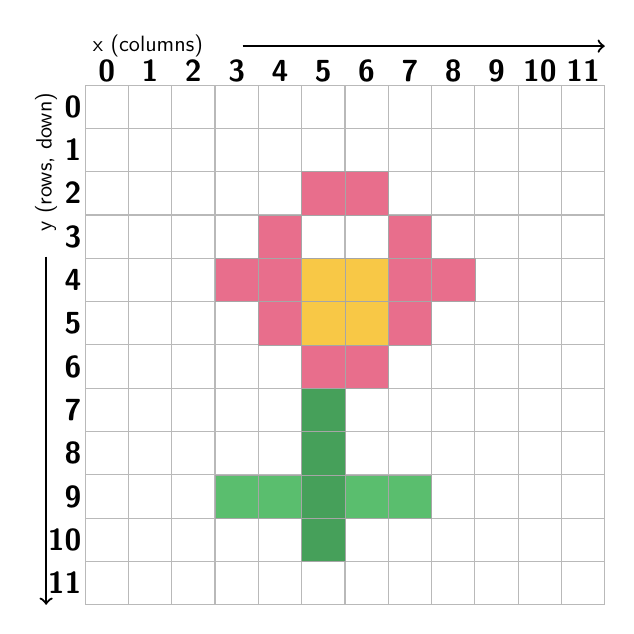
\begin{tikzpicture}[
  font=\sffamily,
  x=0.55cm, y=0.55cm, % pixel size
  line join=round
]
  % ---- grid size ----
  \def\W{12} % number of columns
  \def\H{12} % number of rows

  % ---- background ----
  \fill[white] (0,0) rectangle (\W,\H);

  % ---- draw grid ----
  \draw[step=1, gray!55] (0,0) grid (\W,\H);

  % ---- axis labels: x left->right, y top->bottom ----
  % Column indices along top: 0..W-1
  \foreach \x in {0,...,11} {
    \node[anchor=south, scale=1.1, font=\bfseries\sffamily, inner sep=1pt] at (\x+0.5, \H) {\x};
  }
  % Row indices along left, with y increasing downward:
  % Put 0 at the top row (near y=H-0.5), then 1 below it, ...
  \foreach \y in {0,...,11} {
    \node[anchor=east, scale=1.1, font=\bfseries\sffamily, inner sep=1pt] at (0, \H-\y-0.5) {\y};
  }

  % Optional axis titles
  \node[anchor=west, scale=0.8] at (0, \H+0.9) {x (columns)};
  \draw[->,line width=0.8pt] (2cm, \H+0.9) -s (\W,\H+0.9);
  \node[anchor=east, scale=0.8, rotate=90] at (-0.9, \H) {y (rows, down)}; % name this node Y
  \draw[->,line width=0.8pt] (-0.9, \H+4cm) -- (-0.9, 0); % start this at the south of Y offset by 0.5 downwards and continue it down

  % ---- helper: draw a pixel at (x,y) where y=0 is top row ----
  % We'll just place rectangles manually using the mapping:
  % pixel (x,y) -> rectangle from (x, H-y-1) to (x+1, H-y)

  % Colors
  \definecolor{petal}{RGB}{232,110,140}
  \definecolor{center}{RGB}{248,200,70}
  \definecolor{stem}{RGB}{70,160,90}
  \definecolor{leaf}{RGB}{90,190,110}

  % ---- flower pixels ----
  % petals (a chunky 5x5-ish flower head)


  % Petals (explicit, simpler)
  \foreach \x/\y in {
    5/2, 6/2,
    4/3, 7/3,
    3/4, 8/4,
    4/5, 7/5,
    5/6, 6/6,
    5/4, 6/4, 4/4, 7/4 % make it fuller
  }{
    \fill[petal] (\x, \H-\y-1) rectangle (\x+1, \H-\y);
  }

  % center
  \foreach \x/\y in {5/4,6/4,5/5,6/5} {
    \fill[center] (\x, \H-\y-1) rectangle (\x+1, \H-\y);
  }

  % stem
  \foreach \x/\y in {5/7,5/8,5/9,5/10} {
    \fill[stem] (\x, \H-\y-1) rectangle (\x+1, \H-\y);
  }

  % leaves
  \foreach \x/\y in {4/9,3/9,6/9,7/9} {
    \fill[leaf] (\x, \H-\y-1) rectangle (\x+1, \H-\y);
  }

  % ---- optional: outline the flower pixels slightly darker ----
  \foreach \x/\y in {
    5/2, 6/2,
    4/3, 7/3,
    3/4, 4/4, 5/4, 6/4, 7/4, 8/4,
    4/5, 5/5, 6/5, 7/5,
    5/6, 6/6,
    5/7,5/8,5/9,5/10,
    4/9,3/9,6/9,7/9
  }{
    \draw[black!35, line width=0.2pt] (\x, \H-\y-1) rectangle (\x+1, \H-\y);
  }

\end{tikzpicture}

 \par
    \captionof{figure}{Just like we can refer to any point on a line by
      a number, we can refer to any point on a rectangle or grid using
      two numbers. In this image of a flower, we can use cartesian
      coordinates to reference any square and change its color or turn
      it on or off.}
    \label{fig:cartesian-grid}
  }
}

\subsection{Drawing Our First Image}

In order to draw on a computer, we have to first think about what sort of \emph{language} we need to
use to be specific about what to draw. Once such language is called Turtle.

Turtle works by following -- you guessed it -- rules! Turtle works like an Etch-a-sketch. You supply
instructions that move a pen around a page. Turtle draws a line as the pen moves.

\begin{marginfigure}
  \centering
  \includegraphics[width=0.9\textwidth]{../week2/figures/Jack_of_hearts.jpg}
  \caption{The Turtle language works like an Etch-a-sketch. A pen moves around the page leaving marks that turn into images, such as this one.\attribution{By Etcha - Own work, CC BY-SA 3.0, https://commons.wikimedia.org/w/index.php?curid=5395767}}
  \label{fig:etchasketch}
\end{marginfigure}

% TODO Setup course materials

We're going to use a version of Turtle that is a bit more intuitive than ``standard'' Turtle. This
is provided as part of the course materials in the form of a \term{module}, which is a re-usable
bundle of Python code. In order to use this version, we will have to load it into Python. We can do
this with the \kw{import} rule.

We don't need to know all the details to use it. \curious{Check out \prettyref{fig:import} for a
  complete rundown of \kw{import}.} Let's go ahead and load Turtle and draw our first shape: a line.

\begin{figure}[b]
  \centering
  \begin{minipage}{0.9\textwidth}
    \Large \ttfamily
    \vspace{1.5cm}
    \begin{tcolorbox}[sharp corners]
      \tikzmarknode{importkw}{\kw{import}} \tikzmarknode{import module name}{week2.draw} \tikzmarknode{aspart}{\kw{as} draw}
    \end{tcolorbox}
    \vspace{3cm}
    \begin{tcolorbox}[sharp corners]
      \tikzmarknode{fromkw}{\kw{from}} \tikzmarknode{from import module name}{week2.draw} \tikzmarknode{import from}{\kw{import}} \tikzmarknode{import from star}{*}
    \end{tcolorbox}
  \end{minipage}
  \begin{tikzpicture}[remember picture, overlay]
    \node[above] (importkwnote) at ($(importkw) + (1cm, 1.5cm)$) {
      \begin{tcolorbox}[code note]
        \footnotesize \sffamily
        The \kw{import} rule tells Python to start loading a module.
      \end{tcolorbox}
    };
    \node[below] (import module name note) at ([xshift=-1cm, yshift=-1cm]import module name.south) {
      \begin{tcolorbox}[code note]
        \footnotesize \sffamily
        This is the name of the ruleset or \term{module} we want to use.
      \end{tcolorbox}
    };
    \node[anchor=north west] (aspartnote) at ([yshift=-0.6cm]aspart.south west) {
      \begin{tcolorbox}[code note, width=5cm]
        \footnotesize \sffamily
        This \emph{names} the module. We can refer to rules in the
        module as \code{draw.rule}. You can also ignore the \kw{as}
        part, and use the full name \code{week2.draw.rule}.
      \end{tcolorbox}
    };
    \draw[->, ultra thick] (importkwnote.south) to[in=90,out=-90] ([yshift=1em]importkw.north);
    \draw[->, ultra thick] (aspartnote.north) to[in=-90,out=90] (aspart.south);
    \draw[->, ultra thick] ([yshift=0.2ex]import module name note.north) to[in=-90,out=90] ([yshift=-0.5em]import module name.south);
    \draw[->, ultra thick] ([yshift=-0.2ex]import module name note.south) to[in=90,out=-90] ([yshift=2em]from import module name.north);
  \end{tikzpicture}
  \caption{The \kw{import} rule in Python lets you use extra sets of functionality that are not
    built-in to Python. It takes the name of a module, which is a series of words, separated by
    dots. You also specify how you want to refer to the rules contained in that module, after
    \kw{as}. If you don't include \kw{as}, you have to use the full name of the module.

    You can also get all the rules from a module using the \kw{from} / \kw{import} rule.
  }
  \label{fig:import}
\end{figure}

\begin{replbox}
>>> (*@\tikzmarknode{import keyword}{\kw{import}}@*) week2.draw as (*@\tikzmarknode{week2 draw name}{draw}@*)<ENTER>
>>> draw.draw(draw.forward(100))<ENTER>
\end{replbox}

What happened here? The pen started in the middle of the page, and then went \emph{forward} by 100
units.\curious{The units used by Turtle are called \term{pixels}. See \prettyref{fig:pixels} for
  more information} In this case, the pen always starts pointed to the right. So when we go forward,
turtle draws a line to the right.

Let's break it down further though. There are actually \emph{two} rules being used here. The first
is \code{draw.draw}. This rule takes a drawing and draws it. It doesn't draw anything on its own. If
you just did the following, you'd get a blank screen:

\begin{replbox}
>>> draw.draw()<ENTER>
\end{replbox}

You need to make a drawing in order for \code{draw.draw} to do something. This is what the
\code{draw.forward} rule does. Go ahead and try this:

\begin{replbox}
>>> draw.forward(10)<ENTER>
[('forward', 10)]
\end{replbox}

That didn't draw anything! That's because the \code{draw.forward} rule only describes \emph{what} to
draw. It doesn't do any drawing yourself. You need to ask Python to draw the drawing you create.

Now that we understand the difference between doing the drawing and planning the drawing, let's talk
about what we can do with the plans.

The simplest thing we can do with drawing plans is to combine them together in sequence -- first
make one drawing, then the other. You can put drawings together by using \code{+}, just like you can
with numbers. Let's try this:

\begin{replbox}
>>> draw.forward(10) + draw.turn('right') + draw.forward(20)<ENTER>
[('forward', 10), ('right', 90), ('forward', 20)]
\end{replbox}

Again, that's just the \emph{plan} for the drawing. It doesn't \emph{do} anything until you draw
it. Let's try drawing it:

\hint{For a full explanation of \code{draw.turn}, see \prettyref{deepdive:draw-turn-angles}}
\begin{replbox}
>>> draw.draw(draw.forward(10) + draw.turn('right') + draw.forward(20))<ENTER>
\end{replbox}

That's more like it.

What we saw above is the distinction between \term{data} and
effects. Data is information about something. Data describes what
something is. The \code{draw.forward} and \code{draw.turn} rules made
\emph{data}. The \code{draw.draw} rule used that data to make a
drawing.\didyouknow{The difference between data and effects is similar
  to the difference between \emph{nouns} and \emph{verbs}. Nouns don't
  do anything on their own. They're just there. You need a verb to do
  something with it.}

\subsection{More Complex Drawings}

\curious{For a full list of all the Turtle rules we can use see \prettyref{tab:turtle}.}
Let's try changing the pen color using the \code{draw.color} rule.

\hint{For a sample list of colors we can use, see \prettyref{fig:turtlecolors}}
\begin{replbox}
>>> draw.draw(draw.color('blue')+draw.forward(100))<ENTER>
\end{replbox}

Did it do what you thought it would?

You've seen how to turn the pen above to draw a corner. We can go ahead and extend that to draw a square.

\begin{marginfigure}
  \centering
  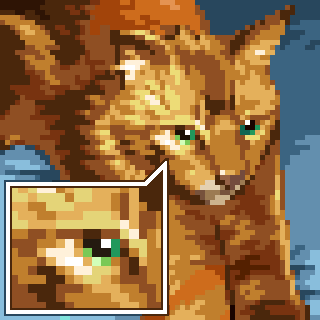
\includegraphics[width=0.9\marginparwidth]{../week2/figures/CatPixels.pdf}
  \caption{Every image you see on a computer screen is made up of tiny lights called \term{pixels}
    arranged in a grid. If you carefully look at your computer screen, you may be able to see the
    individual pixels. By turning the lights on and off and adjusting the color, the computer can
    display any image, such as this one of a cat.  \attribution{Original: ReffPixels?Vector:
      OmegaFallon, CC BY-SA 4.0 <\url{https://creativecommons.org/licenses/by-sa/4.0}>, via
      Wikimedia Commons}}
  \label{fig:pixels}
\end{marginfigure}

\tikzforeground{
  \node (repl dots hint) at ($(repl dots.north east) + (8cm, 2cm)$) {
    \begin{tcolorbox}[code note]
      If we don't complete our rule on the \code{{>}{>}{>}} line, Python will respond with these dots to
      ask us to complete the rule. It tries to be nice that way!
    \end{tcolorbox}
  };
  \draw[->] (repl dots hint.south) to[in=-20,out=-90,looseness=0.6] (repl dots.south east);
}
\begin{replbox}
>>> draw.draw(draw.color('blue') +
...  draw.forward(100) +
...  draw.turn('right') +
...  draw.forward(100) +
...  draw.turn('right') +
...  draw.forward(100) +
...  draw.turn('right') +
(*@\tikzmarknode{repl dots}{...}@*)  draw.forward(100))<ENTER>
\end{replbox}

Phew! That was a lot of typing! If we had to do that everytime we wanted to draw a square, we would
have to write \emph{a lot} of \emph{rules}.

\begin{figure}[b] 
  \centering
  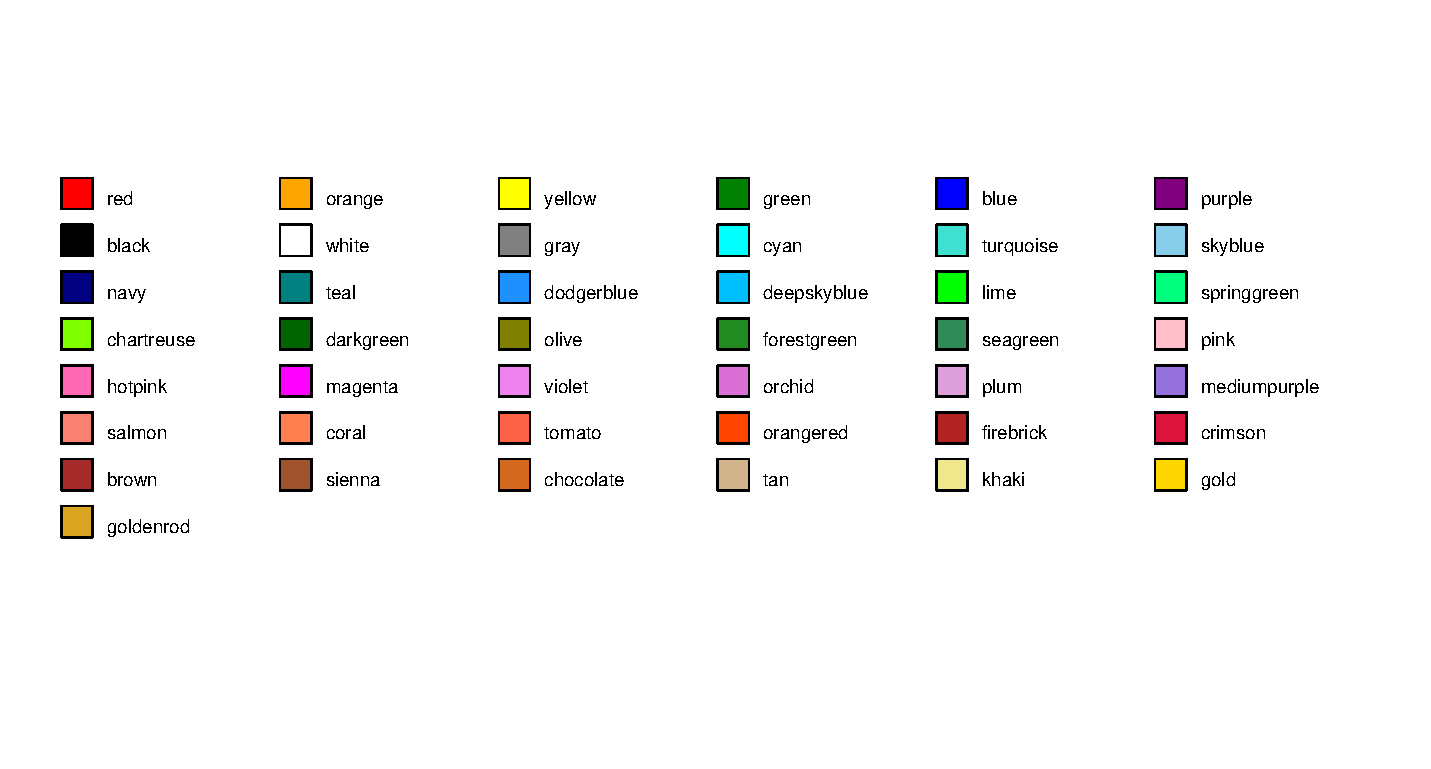
\includegraphics[width=\linewidth, trim={0 3cm 0 3cm}]{../week2/figures/turtle-colors.eps}
  \caption{Some common Turtle colors that you can use. Get creative!}
  \label{fig:turtlecolors}
\end{figure}

\section{Re-using models}

One of the benefits of saving our rules is that we can do the same thing over again. Above, we
created a precise description of a square. Now we need to figure out a way to re-use it.

The first way to re-use rules is to save them into a \term{file}. We call rules that we save on a
computer \term{source code}.

Let's try saving a rule. Open up Thonny and, instead of the prompt, point your mouse at the editor
(\prettyref{fig:thonny-interface}). Rules that we type here can be saved on the computer.
\hint{You can also access all these files on the internet at \url{\giturl}.\\
\begin{center}
\qrcode{\giturl}
\end{center}
}

\hint{Ask your teacher to help you find the \texttt{csforkids} code folder.}
\begin{marginfigure}
  \centering
  \includegraphics[width=0.8\textwidth]{../week2/figures/thonny-run.png}
  \caption{The ``Run'' button at the top of the Thonny interface lets you run code saved in a file.}
  \label{fig:thonny-run}
\end{marginfigure}
\begin{TryThisBox}
  Type the following into the editor and then save it in a file named
  \texttt{duck.py} inside the top-level \texttt{csforkids} folder.

  You can load this file by clicking the green ``Run'' button in the Thonny interface as shown in \prettyref{fig:thonny-run}.
  \begin{lstlisting}
from week2.draw import *<ENTER>
<ENTER>
draw(<ENTER>
  color('blue') +<ENTER>
  forward(100) + turn('right') +<ENTER>
  forward(100) + turn('right') +<ENTER>
  forward(100) + turn('right') +<ENTER>
  forward(100)<ENTER>
)<ENTER>
  \end{lstlisting}
  \tcblower
  You should get something like this:\\
  \includegraphics[width=0.7\linewidth, trim={0 2cm 0 2cm}]{../week2/figures/onesquare.eps}
\end{TryThisBox}

\subsection{Introducing \kw{def}}

That's good, but computers can draw squares without loading
files. This is where the \kw{def} rule come in. Here's how it works.

When we have a bunch of rules we want to re-use, we can use \kw{def} to give a \emph{name} to our
rules. Then, underneath
\kw{def}, we write the rules that make up the new rule. The rules underneath have to be \term{indented}, which means that we have to type two
{\spacekey}s before typing the rule.\curious{Python is known as an \emph{indentation-aware}
language. Some languages do not care about spaces and have other ways to figure out which rules
belong as sub-rules of other rules. But for now, we'll stick with how Python does things!}

\begin{TryThisBox}
  Type the following into \texttt{duck.py}:
  \begin{lstlisting}
def square():
  draw(<ENTER>
    color('blue') +<ENTER>
    forward(100) + turn('right') +<ENTER>
    forward(100) + turn('right') +<ENTER>
    forward(100) + turn('right') +<ENTER>
    forward(100)
  \end{lstlisting}
\end{TryThisBox}

Now try this in the prompt.\hint{Remember to re-run the file (see \prettyref{fig:thonny-run}).}

\begin{replbox}
>>> square()<ENTER>
\end{replbox}

Can we draw two squares? Let's try it?

\begin{replbox}
>>> square()<ENTER>
>>> square()<ENTER>
\end{replbox}

Uh-oh! The second \code{square()} started from a blank screen. This is
because the \code{draw()} rule always starts from a blank
screen. Because we put \code{draw} in our \code{square} rule
above, \code{square} became an action, even though we just wanted the
\emph{data} that was describing our drawing.

Let's be clear about what happened.

\begin{enumerate}
\item You used the \code{square()} rule.
\item Inside \code{square()}, \code{draw()} drew the drawing we gave to it, which is one square on a new blank screen.
\item You used the \code{square()} rule \emph{again}.
\item This caused \code{draw()} to do what it \emph{always} does, which is to create a blank screen and draw a square.
\end{enumerate}

If we want to draw two squares, we're going to have to combine the
rules that just specified the \emph{data} that describes the
square. Let's try it.

\hint{The \code{\textbackslash} at the end of the line means to treat the next line as part of the
  current line. You can skip them if you want and write everything on one line, but such long lines
  won't fit on this page!}
\begin{TryThisBox}
  Type the following into \texttt{duck.py} \begin{lstlisting}
def square_shape():
  color('blue') + \<ENTER>
  forward(100) + turn('right') + \<ENTER>
  forward(100) + turn('right') + \<ENTER>
  forward(100) + turn('right') + \<ENTER>
  forward(100)
  \end{lstlisting}
\end{TryThisBox}

Reload the file by hitting the ``Run'' button and let's try it.

\begin{replbox}
>>> draw(square_shape() + forward(200) + square_shape())<ENTER>
\end{replbox}

Uh-oh! That didn't work. What's going on?

Remember above how the \code{forward()} was a \emph{plan} for a
drawing, but not the drawing itself? We were able to see the plan, by
just using \code{forward()} without \code{draw()}. Let's see
if we can figure out what's going on with \code{square\_shape()}.

First, let's think about what we want. We would want
\code{square\_shape()} to be a drawing plan that went forward four
times, and turned right each time.

Is that what really happens?

\hint{Even though \code{square\_shape()} didn't do what we wanted,
  Python never gave an error. That's because \code{square\_shape()} is
  not an error according to Python. Python just followed its rules
  exactly -- they just weren't the same as the rules we had in mind.}
\begin{replbox}
>>> square_shape()
\end{replbox}

Nothing comes out!

\subsection{The \kw{return} rule}

Here's what's going on. Inside \code{square\_shape()}, we wrote down a
drawing plan, but we never told Python what to do with that plan. In
the prompt, rules that make data cause Python to respond with that
data. Inside a \kw{def}, Python just throws it away, because we didn't
ask Python to keep it.

We use the word \kw{return} inside \kw{def} to say: I've made some data, and this is what I want to
keep. This is the word we need to get Python to keep our plan. Go ahead and modify
\code{square\_shape()}.

\hint{Make sure to pay attention to indentation. You have to add
  spaces in front of \code{forward} in order to keep it ``under''
  the \kw{return}. You can also choose to type it all on one
  line. Remember \code{\textbackslash} is just a convenience.}
\begin{TryThisBox}
\begin{lstlisting}
def square_shape():
  @@return@@ color('blue') + \<ENTER>
    forward(100) + turn('right') + \<ENTER>
    forward(100) + turn('right') + \<ENTER>
    forward(100) + turn('right') + \<ENTER>
    forward(100)
\end{lstlisting}
\end{TryThisBox}

Now, let's see if it does what we expect:

% TODO
\begin{replbox}
>>> square_shape()
\end{replbox}

\begin{BigIdeaBox}
  We can enter as many rules as we want into \kw{def} but we have
  to use \kw{return} if we want Python to respond with particular data.
\end{BigIdeaBox}

\subsection{Combining rules}

Now \code{square\_shape()} results in the drawing plan for a square. Programmers often say that
\code{square\_shape()} \term{evaluates} into the drawing plan for a square, and this is the
terminology we'll use from now on.

We can now use \code{square\_shape()}  with \code{draw()}.

\begin{replbox}
>>> draw(square_shape() + forward(200) + square_shape())
\end{replbox}

And there's two squares!

\begin{bookbox}
\begin{DeepDiveBox}
  \boxtitle{Angles and \code{draw.turn}}
  \label{deepdive:draw-turn-angles}

  \tikzmarknode{angle names}{}
  \code{draw.turn()} \emph{turns} the Turtle cursor. Remember that the cursor is always pointing in
  a particular direction. Turning doesn't cause anything to be drawn, but it does cause future
  \code{draw.forward}s (and other rules) to start off in that direction.

  Angles are measured in \term{degrees}. If you turn 180 degrees (also written as $180^{\circ}$) then
  you turn to face the opposite direction. If you turn 360 degrees (twice 180), then you end up
  facing the same way. By convention, Turtle always turns counter-clockwise, so turning 90 degrees
  (one-half 180) means you end up turning left.

  What if you want to turn right? Remember, you can always turn 180 degrees to turn the other
  direction. From there, turning 90 degrees to the left would leave you facing rightwards of your
  original position. Thus, to turn right, you need to turn 270 degrees. The diagram below shows some
  common angles you might need to know.

  \begin{center}
    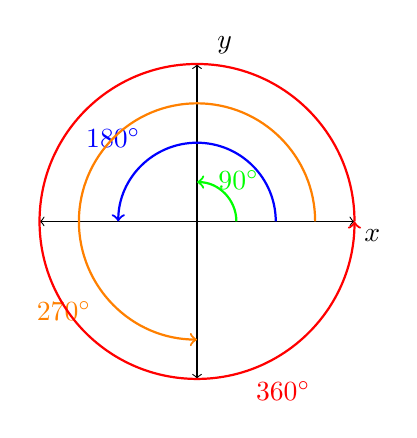
\begin{tikzpicture}
      \draw[<->] (0, -2) -- (0, 2) node[above, xshift=1em] {$y$};
      \draw[<->] (-2, 0) -- (2, 0) node[anchor=west, yshift=-0.5em] {$x$};
      \draw[->, green, thick] (0.5,0) arc (0:90:0.5) node[midway,xshift=0.5em,yshift=0.5em] {$90^{\circ}$};
      \draw[->, blue, thick] (1,0) arc (0:180:1) node[pos=0.7,anchor=south east] {$180^{\circ}$};
      \draw[->, orange, thick] (1.5,0) arc (0:270:1.5) node[pos=0.8,anchor=north east] {$270^{\circ}$};
      \draw[->, red, thick] (2,0) arc (0:360:2) node[pos=0.8,anchor=north west] {$360^{\circ}$};
    \end{tikzpicture}
  \end{center}
\end{DeepDiveBox}
\end{bookbox}
\onfloatpage{deepdive:draw-turn-angles}{
  \makemargmark{angle names}{
    \code{draw.turn()} allows the following angle names as shortcuts:
    \begin{description}
    \item[\kw{'right'}] Turn towards the right
    \item[\kw{'left'}] Turn towards the left
    \item[\kw{'around'}] Turn all the way around so you're facing the opposite direction
    \end{description}
  }
}

\subsection{Complex Rules}

\begin{table*}[t]
  \fixfigure
  \begin{tabular}{p{0.24\linewidth}p{0.76\linewidth}}
    \toprule
    Rule & What it does\\\midrule
    \code{draw.goto(x, y)} & Move the pen to the particular \code{x} and \code{y} coordinate.\\
    \code{draw.forward(x)} & Move forward \code{x} units in the current direction of the pen.\\
    \code{draw.circle(r)} & Draw a complete circle with the given radius \code{r}. \\
    \code{draw.circle(r, p)} & Draw a portion of a circle with radius \code{r}. The \code{p} argument specifies what percent of the circle to draw. For example, \code{p} of 0.5 draws a half-circle. \\
    \code{draw.penup()} & Lift the pen \emph{up}. Future movement commands will not draw anything.\\
    \code{draw.pendown()} & Place the pen back \emph{down}. Future movement commands will draw.\\
    \code{draw.color(c)} & Change the color of the pen.\\
    \code{draw.pensize(s)} & Change the size of the tip of the pen.\\
    \code{draw.fill(c, pic)} & Draw \code{pic} and fill in all enclosed areas with color \code{c}.\\
    \code{draw.turn(angle)} & Turn by the given angle, which can be an angle (in degrees), or \code{``left''} or \code{``right''}. \\
    \code{draw.wait(s)} & Wait \code{s} seconds before proceeding. Let's you see how the drawing progresses. \\
    \code{draw.pause(prompt)} & Pause the drawing and display the word \code{prompt} until the user hits \enterkey \\
    \bottomrule
  \end{tabular}
  \caption[][1ex]{These are all the Turtle rules you can use and combine
    together using functions!}
  \label{tab:turtle}
\end{table*}

Grouping rules in this way is a fundamental part of computer programming. Computer programmers have
special names for rules built using \kw{def} and \kw{return}. We call them
\term{functions}. Functions allow complicated things, like shapes, to be hidden away inside rules
that are easier to understand. Now that you've made a \code{square\_shape()}, you can forget all the
details involved with drawing a square. Whenever you need a square, you can just use
\code{square\_shape()}!

\begin{replbox}
draw.draw(
  draw.color('blue') + square_shape() +
  draw.color('red') + square_shape())<ENTER>
\end{replbox}
% TODO GRAPHICS\includegraphics[width=0.8\linewidth]{../week2/figures/twosquares1.eps}

We did that without ever worrying about exactly \emph{how} the square was drawn.\curious{Much of Python itself is written using \kw{def} and \kw{return}. The rules we make with them are no less real than the rules that come with Python.}

\subsection{Arguments}

One of the limitations of \code{square\_shape()} is that it only draws squares of one size. If we
wanted to draw a square for the duck's body and then a smaller square for the duck's head, then we
would have to write two functions that looked the same, like below:

\begin{TryThisBox}
\begin{lstlisting}
def big_square_shape():
  return color('blue') + \<ENTER>
    forward(200) + turn('right') + \<ENTER>
    forward(200) + turn('right') + \<ENTER>
    forward(200) + turn('right') + \<ENTER>
    forward(200)

def small_square_shape():
  return color('blue') + \<ENTER>
    forward(100) + turn('right') + \<ENTER>
    forward(100) + turn('right') + \<ENTER>
    forward(100) + turn('right') + \<ENTER>
    forward(100)
\end{lstlisting}
\end{TryThisBox}

This would quickly get unwieldy. We used \kw{return} to get data out of our function. Now we need a
way to put data \emph{in}. This is what \term{arguments} are.

Arguments are placeholders for things that we don't know yet. Here's a function that could draw a
square of any size:

\begin{TryThisBox}
\begin{lstlisting}
def square_shape(n):
  return color('blue') + \<ENTER>
    forward(n) + turn('right') + \<ENTER>
    forward(n) + turn('right') + \<ENTER>
    forward(n) + turn('right') + \<ENTER>
    forward(n)
\end{lstlisting}
\end{TryThisBox}

Let's see how to use it:

\mTrackBox{Graphics}{ The sort of drawing we are doing with Turtle is called \term{vector
    graphics}. Vector graphics store details on shapes and colors. Because computers can draw shapes
  at any size, vector graphics can be scaled to any size. Your square could be bigger than your
  classroom!}
\begin{replboxannotated}
>>> draw.draw(
...   draw.color('blue') + square\_shape(100) +
...   draw.color('red') + square\_shape(200))<ENTER>
\tcblower
\includegraphics[trim={0 0 0 3cm}, width=0.8\linewidth]{../week2/figures/twosquares1.eps}
\end{replboxannotated}

There's one problem: all of these programs draw the second square in a different way than the first. The
second square appears on top of the first square, instead of in the same position. What's going on?

\section{Errors with Data}

When we originally wrote \code{square\_shape()}, Python did not make a fuss. However
\code{square\_shape()} did not work the way we expected it to. When our expectation of how things
work does not match what actually happens, we call it a \term{bug}.\didyouknow{The first computers
  stored data using vacuum tubes, which were like lightbulbs that could either be switched on or
  off. Vacuum tubes were large and unwieldy and not as reliable as the computers we use today. The
  warm and bright tubes attracted insects, and these insects would sometimes cause the tubes to
  short-circuit. This is the origin of the word \term{bug}! Yuck!}

The squares appearing atop each other instead of in the same spot is another example of a bug.

We work through errors in a process called \term{debugging}. One of the ways in which we debug is by
asking the program to \emph{stop} before it's completed so we can see what it's doing.

The Turtle library we are using provides a simple way to stop the drawing so we can look at it.

\begin{replbox}
>>> draw.draw(draw.pause('square 1') +<ENTER>
... draw.color('blue') + square_shape(200) +<ENTER>
... draw.pause('square 2') + draw.color('red') +<ENTER>
... square_shape(200)
\end{replbox}

\hint{You can always get back to
  the prompt and quit what you're currently doing by holding down both \controlkey and
  \litkey{C}. This is known as an \emph{interrupt}.}
The \code{draw.pause} rule causes Python to \emph{pause} before each square is drawn and wait for
you to type \enterkey in the prompt before it continues drawing.

You should get something like \prettyref{fig:twosquares-debug}.

\begin{figure}
  \fixfigure
  \label{fig:twosquares-debug}
  \centering
  \begin{minipage}{0.48\linewidth}
    \centering
    \includegraphics[width=\linewidth, trim={0 0 0 4cm}]{../week2/figures/twosquares-debug-square 1.eps}\\
    The First Square
  \end{minipage}
  \hfill
  \begin{minipage}{0.48\linewidth}
    \centering
    \includegraphics[width=\linewidth, trim={0 0 0 4cm}]{../week2/figures/twosquares-debug-square 2.eps}\\
    The Second Square
  \end{minipage}
  \caption{What it looks like before each square is drawn. Can you
    spot the difference?

    \textbf{Hint:} Look at the arrow.}
\end{figure}

What do you notice about the arrow in each picture? In Turtle, this arrow is called the
\emph{cursor} and its direction changes how \code{draw.forward} works. If the arrow is pointing
right, then \code{draw.forward} draws to the right. Similarly, if the arrow is pointing towards the
top, then \code{draw.forward} draws towards the top. If you look at the arrow, you'll notice that,
before the first square, it points right, and before the second, it points upward.

How do we fix this issue? The cursor starts pointing right by default. It points upward after the
first square is drawn using the \code{square} function. How do we get it to point right again? Can
you think of an answer?

\begin{BigIdeaBox}
  Sometimes, when combining programs together, things don't work the
  way we expect because our mental model of how the computer ought to
  have done something doesn't match the exact set of rules the
  computer followed.

  It often helps to use tools like \code{draw.pause} to inspect what
  is happening in the middle of our program.
\end{BigIdeaBox}

Here's the solution (pay attention to the italicized part!)

\begin{TryThisBox}
  \begin{lstlisting}
def square_shape(n):
  return \
    draw.forward(n) + draw.turn('right') + \
    draw.forward(n) + draw.turn('right') + \
    draw.forward(n) + draw.turn('right') + \
    draw.forward(n)@@ + draw.turn('right')@@
  \end{lstlisting}
\end{TryThisBox}

Now, our squares are drawn the same way, but they overlap, just like we expected.

\includegraphics[width=0.8\textwidth, trim={0 0 0 4cm}]{../week2/figures/twosquares-fixed.eps}

\subsection{Going Full Circle}

Squares and lines are interesting, but it would be hard to do a lot of
interesting drawing using just those. Let's look at some other shapes.

The first shape we'll introduce is a \emph{circle}. A circle is defined by its radius, which is half
the total distance across the circle. For example, to draw a circle with a 30 unit radius, we can
use \code{draw.circle(30)}. Try this and see what happens.

\begin{replbox}
  draw.draw(draw.circle(30))
\end{replbox}

But there's more, you can also draw \emph{parts} of a circle. This is
called an \emph{arc}. To draw an arc, you can use
\code{draw.circle(30, 1/2)}, which will only draw \emph{half} the
circle\hint{You can use \code{1/2} or \code{0.5}. Python understands
  both.}

\begin{replbox}
draw.draw(draw.circle(30, 0.5))<ENTER>
draw.draw(draw.circle(40, 1))<ENTER>
draw.draw(draw.circle(20, 1/3))<ENTER>
\end{replbox}

Now, try drawing this figure.

\includegraphics[width=0.5\textwidth,trim={0 3cm 0 0}]{../week2/figures/lrcircle.eps}

Having trouble? Think back to the examples we tried above. Which way
did the arrow move when drawing the circle?

Turtle assumes that when we want a circle, we always want to draw it in this direction
(counter-clockwise). To make it draw in a clockwise direction, we supply it a \emph{negative} radius
(see \prettyref{fig:turtle-circles}). This arrangement where a computer system always does things
one way and requires the programmer to explicitly choose another way is called a \term{default}.

\begin{figure}[p]
  \fixfigure
  \label{fig:turtle-circles}
  \caption{The \code{draw.circle} rule produces some portion of a circle with a particular radius,
    as illustrated above. A positive radius corresponds to a point to the ``left'' of the cursors
    direction. A negative radius means to go to the right.

    The diagram here demonstrates the result of

    \code{draw.circle(30, 0.15) + draw.circle(-15,0.6)}
  }
  \begin{tikzpicture}[font={\sffamily\footnotesize}]
    \pgfmathsetmacro{\angleone}{2 * pi/360 * -100}
    \pgfmathsetmacro{\circleportion}{0.15}
    \pgfmathsetmacro{\circleportiontwo}{0.6}
    \pgfmathsetmacro{\circleportiontworad}{\circleportiontwo * 2 * pi}
    \pgfmathsetmacro{\circleportionrad}{\circleportion * 2 * pi}

    \pgfmathsetmacro{\circleonefinalangle}{\angleone+\circleportionrad}
    \pgfmathsetmacro{\midx}{cos(\circleonefinalangle r) * 2}
    \pgfmathsetmacro{\midy}{sin(\circleonefinalangle r) * 2}
    \pgfmathsetmacro{\circletwox}{cos(\circleonefinalangle r) * 3}
    \pgfmathsetmacro{\circletwoy}{sin(\circleonefinalangle r) * 3}
    \pgfmathsetmacro{\circletwostart}{acos(\midx - \circletwox)}
    \pgfmathsetmacro{\finalx}{\circletwox + cos((\circletwostart + \circleportiontworad) r)}
    \pgfmathsetmacro{\finaly}{\circletwoy + sin((\circletwostart + \circleportiontworad) r)}

    \draw[magenta, thick, dashed] (0,0) circle (2);
    \draw[violet, thick, dashed] (\circletwox,\circletwoy) circle(1);

    \draw[->,dashed,color=IdeaBlue] ({cos(\angleone r) * 2}, {sin(\angleone r) * 2}) -- (0, 0);
    \draw[->,dashed,color=IdeaBlue] (\finalx, \finaly) -- (\circletwox, \circletwoy);

    \draw[decorate, decoration={brace, amplitude=5pt, mirror, raise=0.2em}] (0,0) -- ({cos(\angleone r) * 1.9}, {sin(\angleone r) * 1.9}) node[midway, xshift=-2.1em] {$r = 30$};
    \draw[decorate, decoration={brace, amplitude=5pt, raise=0.3em}] ({\finalx * 0.98}, {\finaly * 0.98}) -- (\circletwox, \circletwoy) node[midway, xshift=-1.5em, yshift=-1.5em] {$r = -15$};

    \draw[black, ultra thick, {Stealth[reversed]}-{Stealth}] ({cos(\angleone r) * 2}, {sin(\angleone r) * 2}) arc ({deg(\angleone)}:{deg(\circleportionrad + \angleone)}:2) node[midway,name=arc] {};
    \draw[black, ultra thick, {Stealth-}] (\finalx,\finaly) arc
                                                    ({deg(\circletwostart+\circleportiontworad)}:{deg(2 * pi + \circletwostart) + 13}:1) node[midway,name=arctwo]{};
    \draw[dashed,xshift=0.3em,yshift=-0.3em, <-] (arc) to [bend left] ++(-2em, -4em) node[below] {\texttt{draw.circle(30, \circleportion)}};
    \draw[dashed,xshift=0.3em,yshift=0.3em, <-] (arctwo) to [bend right] ++(4em,2em) node[above] {\texttt{draw.circle(-15, \circleportiontwo)}};

\end{tikzpicture}

\end{figure}

To draw the diagram, use this code:
\curious{Try using \code{draw.pause} to visualize exactly which
  portion is drawn by which command!}
\tikzforeground{
  \coordinate (immediate note middle) at ($(immediate note target)!0.5!(immediate note target end)$);
  \node[anchor=west] (immediate note hint) at ([xshift=0.7cm,yshift=-0.2cm]current page text area.east|-immediate note middle) {
    \begin{tcolorbox}[code note]
      You can set \code{immediate=True} to just get the final output, without having to watch Turtle draw.
    \end{tcolorbox}
  };

  \draw[->] (immediate note hint.west) to[out=180,in=-40,looseness=0.8] ($(immediate note target)!0.8!(immediate note target end)$);
}
\begin{replbox}
>>> draw.draw(draw.circle(30, 1/2) + draw.circle(-30, 1/2), (*@\tikzmarknode{immediate note target}{}@*)immediate=True(*@\tikzmarknode{immediate note target end}{}@*))
\end{replbox}

With these shapes, we can make more complicated figures. There's just
one thing left: filling our shapes with color.

We saw how to change the color of the lines we drew, but how do we
\emph{fill} the shapes we draw with a color?

The \code{draw} module provides the \code{draw.fill} rule to create
filled diagrams. Let's try it.

\begin{replbox}
>>> draw.draw(draw.fill('blue', square_shape(100)))<ENTER>
\end{replbox}

\section{The Duck Challenge}

\hint{Start by getting the basic shapes. Then change lengths and measures until it's just right. Try it!}
Remember how we started class by drawing a duck and attempting to describe it to our friend? At that
point we lacked a proper language to talk about drawings. But now we have a way to talk about
drawings precisely! Take a look at your drawing, and break it up into \emph{rules}: lines, circles, etc.
\didyouknow{One of the earliest kinds of computers was known as the
  \textbf{Jacquard Loom}. It revolutionized the manufacture of complex
  patterns in cloth. Weavers would punch cards giving the machine
  directions to raise or lower threads to create complex patterns.

  \begin{center}
    \includegraphics[width=0.9\linewidth]{../week2/figures/Jacquard.loom.cards.jpg}
  \end{center}
}
\begin{TryThisBox}
  Try using what you've learned thus far to draw a duck using \kw{def} and \kw{return} and
  Turtle. Name your function \code{duck}.

  As you're doing this, try to keep re-usable parts of your duck in separate functions, so you don't
  have to figure out the same code over and over again
\end{TryThisBox}

Here are some examples of what you may have created. All of these are examples of a ``duck'' that
you can make using the simple rules for drawing we learned above.

\begin{BigIdeaBox}
  To the computer, there is no duck. It's just a set of rules you told it to follow to draw one
  depiction of a duck that you found useful. We have tonundeesrand the problems we are trying to solve precisely to program them into a conputer.
\end{BigIdeaBox}

\section{Copying Ducks}

You've now drawn \emph{one} duck; what if we wanted more? The whole point of this was to codify
exactly how to make a duck and explain that precisely. Now, with these instructions in hand,
we can make more ducks.

\begin{replbox}
>>> from week2.examples import *<ENTER>
>>> lake_of(duck)<ENTER>
\end{replbox}

Nice! Look at all those ducks. But, there's one problem... all our ducks look the same. Can we make
each one a bit more unique?
\mTrackBox{Music \& Sound}{ We've seen how computers represent images as
  lights going on and off, but how do they represent \emph{sound}?

  When our ears hear sound, they are responding to \emph{changes} in
  air pressure.

  Computers represent this -- you guessed it -- using numbers!

  With graphics, we had to break up the rectangular screen into small
  chunks called pixels. For sound, we instead break up \emph{time}
  into really small sections (tens of thousands per second!) called
  samples. Within each sample, we store a number which represents how strong the sound is at that time. The samples
  are sequenced together rapidly using a componenty called a DAC or
  \term{digital-to-analog converter} and sent to a speaker, which outputs a very short sound at that strength. This process happens tens of thousands of times in one second. Our ear perceives it as high quality sound. }


Let's add some \term{arguments} to our \code{duck} function. Modify
your function to include some arguments.  \hint{The \code{lake_of}
  function supports \code{body_color}, \code{eye_color}, and
  \code{size}, and will use whatever arguments your function has. The
  colors can be used however you want, and the size just says how
  ``big'' to draw the duck. Try it and see!}
\begin{TryThisBox}
  \begin{lstlisting}
def duck(@@body_color@@, @@eye_color@@):
  @@your code@@
  \end{lstlisting}
\end{TryThisBox}

Now, take these arguments and use it to change your duck's body and eye color using the
\code{draw.color} and \code{draw.fill} functions we saw above.

Now, rerun the example above:

\begin{replbox}
from week2.examples import *<ENTER>
lake_of(duck)
\end{replbox}

Much better!

\begin{BigIdeaBox}
  Since we packaged our duck into a function and added arguments to allow certain parts to change,
  we made it trivial to re-use our duck many times. This is a foundational part of computer
  programming.
\end{BigIdeaBox}

\section{Conclusion: From Drawing to Computation}

In this lesson we learned that we can often do things by hand that
take effort to describe to the computer. This is because computers are
precise and follow fixed rules. Once we are able to describe things
precisely, then we can describe them to a computer and manipulate
them. Python lets us store descriptions in \term{source code} or in
\term{functions} which we write using \kw{def} and \kw{return}.

Everything in computer science is a description of something real
(whether a physical item or a real problem) that we want to solve. To
be able to manipulate things with computers we have to be able to
express our problem as rules the computer understands. In the case of
visual information, it means understanding graphics like the Turtle
system. Even though the computers don't \emph{understand} what a duck
is, we were able to describe a drawing of a duck to the computer. In
the next chapters, we'll explore other ways of describing the world to
a computer.

\Exercises

\begin{exercises}
\item Try creating some other animal as a Python function, and using
  it with the \code{lake\_of} function we used before. What does this
  show about Python's \emph{understanding} of the thing we drew?
  \answer{Whichever animal we draw, Python and the lake\_of
    function treat it the same way. Each animal is just a rule
    for Python to draw.}

\item A \emph{regular} polygon is a shape with some number of sides whose sides are all of equal
  lengths. Can you think of a way to write a function that represent a drawing of a regular polygon
  of any number of sides? For example, an equilateral triangle (see below) is the simplest
  polygon. It has three sides, all of the same length. How would you draw this in Turtle? What about
  a square? A pentagon? A hexagon?

  \hintnote The sum of all angles in any polygon sum to $180(n - 2)$, where $n$ is the number of
  sides. So the angles of a triangle always sum to $180(3 - 2) = 180$ degrees.

  \begin{center}
  \begin{tikzpicture}
    \coordinate[label=left:$A$]  (A) at (0,0);
    \coordinate[label=right:$B$] (B) at (4,0);
    \coordinate[label=above:$C$] (C) at (2,3.464);

    \coordinate[label=below:$c$](c) at ($ (A)!.5!(B) $);
    \coordinate[label=left:$b$] (b) at ($ (A)!.5!(C) $);
    \coordinate[label=right:$a$](a) at ($ (B)!.5!(C) $);

    % angle alpha
    \draw[fill=green!30] (0,0) -- (0:0.75cm) arc (0:60:.75cm);
    \draw (0.36cm,0.25cm) node {\small $60^{\circ}$};

    % angle beta
    \begin{scope}[shift={(4cm,0cm)}]
      \draw[fill=green!30] (0,0) -- (-180:0.75cm) arc (180:120:0.75cm);
      \draw (150:0.5cm) node {\small $60^{\circ}$};
    \end{scope}

    % angle gamma
    \begin{scope}[shift={(60:4)}]
      \draw[fill=green!30] (0,0) -- (-120:.75cm) arc (-120:-60:.75cm);
      \draw (-90:0.5cm) node {\small $60^{\circ}$};
    \end{scope}

    % the triangle
    \draw [line width=1.5pt] (A) -- (B) -- (C) -- cycle;
  \end{tikzpicture}
  \end{center}
\item An animation is a series of still images. The \code{lake\_of} function uses your duck function
  to create a simple animation of ducks swimming in a lake. You can do the same thing using
  \code{draw.draw()} function with \code{immediate=True} and the \code{draw.wait} function. Try it!
\end{exercises}

% Show red and blue yin/yan thing
% # ============================================================
% # Chapter 2 TODO Outline (Technical-first)
% # ============================================================
% 
% * Drawing Primitives (Missing Technical Core) - Done
% - Introduce arcs / circles as drawing primitives - Done
% - Show how arcs differ from straight lines - Done
% - Explain radius + angle intuitively (no formulas yet) - Need to ADD diagram
% - Add example: combining lines + arcs -- NOT DONE
% - Add figure showing arc parameters visually -- TODO
% 
% * Filling and Regions -- DONE
% - Introduce closed shapes -- TODO
% - Explain what ?inside? vs ?outside? means -- TODO
% - Introduce fill as coloring a region - DONE
% - Show same outline with and without fill - Add diagram TODO
% 
% * Multiple Duck Representations (Technical)
%     - Draw duck using only lines
%     - Draw duck using lines + arcs
%     - Draw duck using fill
% - Compare versions side-by-side
% - Ask: what details were added / removed?
% 
% * Modeling Choices -- will not do
% - Explicitly name ?model? at this point
% - Identify what each duck drawing ignores -- figure caption
% - Identify what each drawing keeps -- figure caption
% - Add diagram: same duck, different models
% 
% * Simulation: A Lake of Ducks
% - Introduce idea of many ducks, same rules -- done
% - Add simple rule-based placement (position, size, direction)
% - Show variation via parameters -- done
% - Simulate multiple ducks on a lake
% - Add figure: single duck vs many ducks
% 
% * Abstraction via Parameters -- colors of body, and eyes
% - Name parameters explicitly -- 
% - Show how changing numbers canges appearance -- TODO
% - Connect parameters to ?knobvs? on the model -- no
% 
% * From Drawing to Computation
% - State: computer draws by following rules
% - Emphasize repeatability
% - Emphasize no understanding of ?duck?
% 
% * Curiosity / Track Boxes (Insert Where Natural)
% - Graphics: circles aren?t really circles
% - Games: fake physics
% - Sound: sound as numbers
% - Simulation: same rules, many agents
% 
% * Conceptual Wrap-Up
% - Revisit duck question one last time
% - State: model ? thing
% - State: computers work only with models
% - End with forward-looking question
% 
% # ============================================================
